\subsection{Mechanical Trade Studies}
%----------------------------Architecture----------------------
\subsubsection{Architecture}
\label{sect:architectureto}
To perform operations such as Outpost reconfiguration, and capturing and berthing of free flyer, the robotic system needs to have wide workspace range. The arm design that was used for Canadarm and Canadarm2 is capable of these operations. Using this design as reference, three alternative architectures are proposed. 

\begin{enumerate}
\item{\textbf{4 DOF robotic arm with 4 booms and 3 end effector}\\
The first design has 14 joints as shown in \Cref{fig:14dof} below. The two booms at the bottom act as legs to maneuver around the Outpost. The end effectors connected to each legs can grapple to the Outpost and to the free flyer vehicles. There is a smaller arm connects to the elbow joints of the legs, which has 7 DOF to perform inspection, maintenance and repair of the Outpost.
\begin{figure}[H]
\centering
%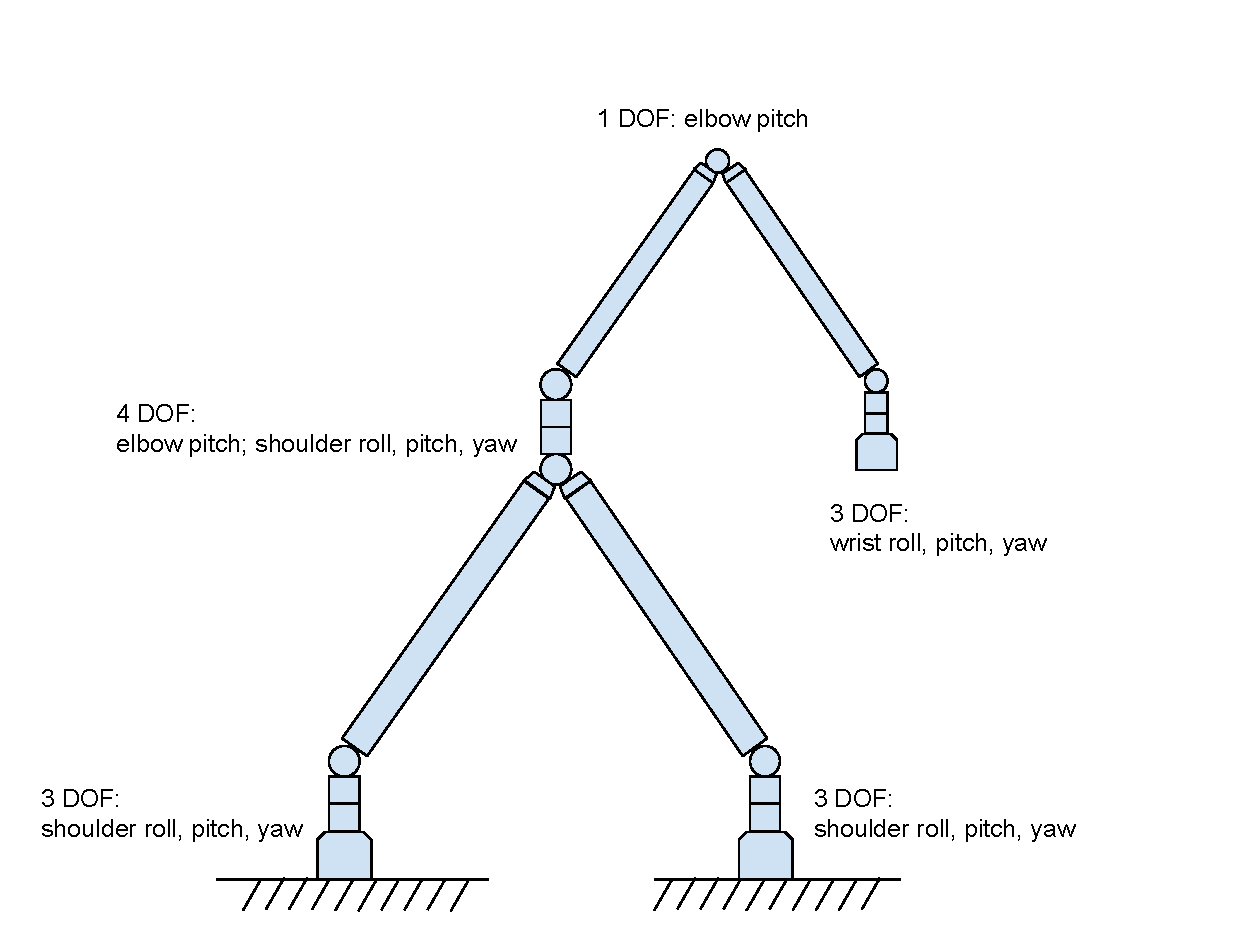
\includegraphics[width=0.5\textwidth]{14dof}
\caption{Sketch of 14DOF arm}
\label{fig:14dof}
\end{figure}
}
\item{\textbf{7 DOF robotic arm with 2 telescopic booms and 2 end effectors}\\
This architecture has two telescopic booms that would be extended once the robotic system is unstowed. The telescopic booms are extended by first connecting both end effectors on the Outpost and allowing the shoulder joint to freely rotate. Then, the elbow joint will rotate and extend the telescopic boom and two booms will extend separately.

The end effectors can grapple to Outpost to perform Outpost reconfiguration as well as free flying vehicles for capture and berthing. The end effectors can also connect to tools that are used for Outpost inspection and maintenance. The sketch of the architecture is shown in \Cref{fig:7dof} below.
\begin{figure}[H]
\centering
%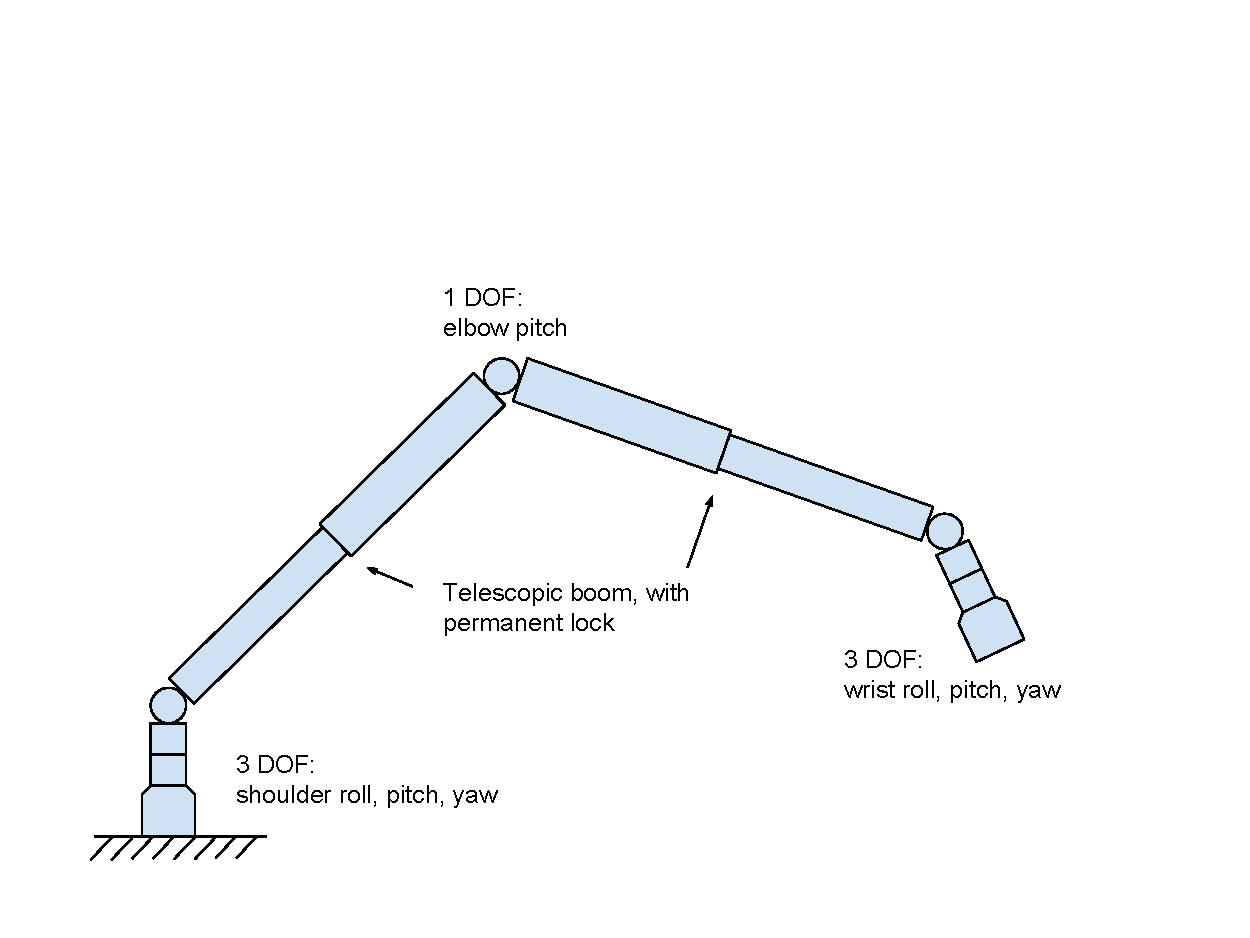
\includegraphics[width=0.55\textwidth]{7dof}
\caption{Sketch of 7DOF arm}
\label{fig:7dof}
\end{figure}
}
\item{\textbf{14 DOF robotic arm with truss rail, 2 booms and 2 end effectors}\\
As shown in \Cref{fig:14dof_truss} below, this design is composed of two parts. The first part is a 8 DOF arm with a truss rail and two booms. The end effectors can grapple to the Outpost to maneuver the robotic arm around the Outpost and perform Outpost reconfiguration. The end effectors can also grapple to free flyingr vehicles for capture and berthing operations. For inspection, maintenance and repair operations, two end effectors will be fixed on the Outpost and the truss rail between two elbow joints will act as guides for the fine arm.

The fine arm has 6 DOF and can move on the truss rail to perform inspection, maintenance and repair operations. Different tools can be attached to the end of the fine arm for specific tasks.
\begin{figure}[H]
\centering
%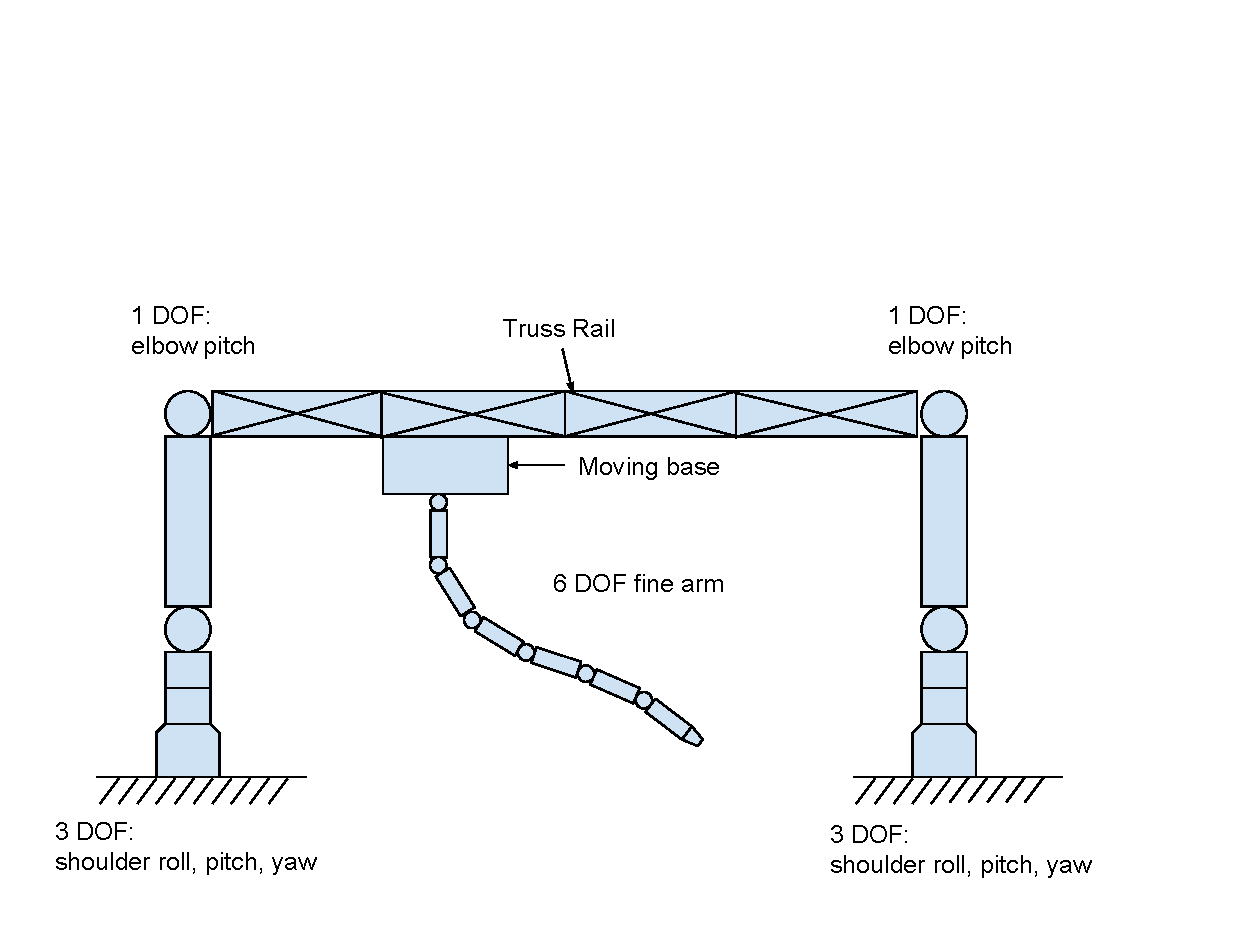
\includegraphics[width=0.6\textwidth]{14dof_truss}
\caption{Sketch of 14DOF arm with truss}
\label{fig:14dof_truss}
\end{figure}
}
\end{enumerate}

\begin{table}[H]
\centering
\caption{Trade Study of Architecture}
\begin{tabular}{|P{2.5cm}|P{4.1cm}|P{4.1cm}|P{4.0cm}|}
\hline
	&	\textbf{Architecture \#1}	&	\textbf{Architecture \#2}	&	\textbf{Architecture \#3}	\\\hhline{|=|=|=|=|}
\textbf{Structure Stability}	&
\textcolor{OliveGreen}{Robot has two fixed points on the Outpost, providing more stability}	&
\textcolor{red}{Robot has only one point fixed to the Outpost, arm will vibrate easily}	&
\textcolor{OliveGreen}{Robot has two fixed points on the Outpost, providing more stability}	\\\hline
\textbf{System Complexity}	&
\textcolor{red}{High complexity due to 14 degrees of freedom [Fund Robo]}	&
\textcolor{OliveGreen}{Lower complexity due to less degrees of freedom, heritage from Canadarm2}	&
\textcolor{red}{High complexity due to 14 degrees of freedom [Fund Robo]}	\\\hline
\textbf{Mass Required}	&
\textcolor{red}{Heaviest out of three due to 14 joints in total [That ERA thing]}	&
\textcolor{OliveGreen}{Lightest out of three\newline Least number of joints}	&
\textcolor{orange}{Medium: Has 8 joints and mechanical parts related to fine arm}	\\\hline
\textbf{Volume Occupied}	&
\textcolor{red}{Large volume due to more booms in the system}	&
\textcolor{OliveGreen}{Least volume out of three: 2 telescopic booms that are retracted in launch position}	&
\textcolor{red}{Large volume due to addition of truss and a fine arm}	\\\hline
\textbf{System Range}	&
\textcolor{orange}{Short range due to relatively shorter boom}	&
\textcolor{OliveGreen}{Long range due to telescopic boom that will extend}	&
\textcolor{orange}{Short range due to relatively shorter boom}	\\\hline
\textbf{Dexterous Tasks}	&
\textcolor{OliveGreen}{High stability due to smaller dexterous arm}	&
\textcolor{orange}{System can attach to tool for dexterous task\newline Low stability}	&
\textcolor{OliveGreen}{System has small dexterous arm\newline High stability}	\\\hline
\end{tabular}
\label{table:architectureto}
\end{table}

%----------------------------Material---------------------------
\subsubsection{Material of Frame}
\label{sect:materialto}
The material of the frame is directly related to the mass and shape of the system. Certain materials are too brittle to manufacture in desired shapes, and will aect the architecture of the system. As the material heavily aects mechanical aspects of the design, trade study on the material of frame was conducted. Material with low density, low coecient of thermal expansion, and high strength are desired for the frame of the system. Commonly used materials in the space industry include carbon bre, aluminum, stainless steel, and titanium. Each material has numerous variations with dierent properties and name. A trade study between four materials were conducted in table below.

\begin{table}[H]
\centering
\caption{Trade Study for type of Thermal Control System}
\begin{tabular}{|P{3.6cm}|P{3.1cm}|P{2.4cm}|P{2.3cm}|P{2.5cm}|}
\hline
	&	\textbf{PAN (Polyacrylonitrile) Carbon Fiber, Aerospace \cite{carbonfibreprop}}	&\textbf{Aluminium 7075 \cite{alumniumprop}}	&	\textbf{Stainless Steel 304 \cite{steelprop}}	&	\textbf{Titanium (Ti-6A/4V) \cite{titaniumprop}}	\\\hhline{|=|=|=|=|=|}
\textbf{Density (\si{\kilo\gram\per\metre\cubed})}	&	
1.8	&	2.81	&	8	&	4.43	\\\hline
\textbf{Ultimate Tensile Strength (\si{\mega\pascal})}	&
3450 to 5520	&	572	&	505	&	900 to 100	\\\hline
\textbf{Thermal Coefficient of Expansion (\si{\micro\metre\per\metre\per\kelvin})}	&	
-0.4 to -0.75	&	23.6	&	17.3	&	8.6	\\\hline
\textbf{Young's Modulus (\si{\giga\pascal})}	&
220 to 448	&	71.7	&	193 to 200	&	113.8	\\\hline
\end{tabular}
\label{table:materialto}
\end{table}

The specific properties of carbon fiber will vary with orientation and volume of the fibers and type of resin used. Aerospace grade carbon fiber, which has high stiffness to weight ratio, were selected for comparison. Other space robotic arms, such as Canadarm, Canadarm2, and ERA are made of carbon fiber as well. In general, carbon fiber is much lighter than titanium and stainless steel, have lower magnitude of thermal coefficient of expansion, and higher young’s modulus and tensile strength. Overall, aerospace grade carbon fiber is the most desirable option out of the four.

%----------------------------End Effector---------------------------
\subsubsection{End Effector}
\label{sect:endeffectorto}
In order to interact with the external subsystems situated around EML2, including the Outpost, astronauts and other modules during various operations, an end effector subsystem is required to build connections with the Outpost and other modules. And the interface established by the end effector shall capable of providing power and data connections to and from the robotic system.

As a result of those criteria, two potential end effector models are listed and compared below:

\textbf{Three fingers-three petals End Effector}: There are two main subassemblies of this end effector: an active mechanism, which consists of a motor driven lead screw that would accurate the linkages between the three finger and three petals; a passive structure, whose geometry will allow it to be constrained by the linkages and therefore establishing a rigid interface.	\\
\textbf{Steel cable-snared End Effector}: This end effector system consists of the snaring and rigidizing subassembly inside the shell, and four latch/umbilical subassemblies outside the shell, which are responsible for the rigidizing loop and the connecting loop after the fine positioning for latching and connecting operation is reached.

\begin{longtable}{|P{2.5cm}|P{6.35cm}|P{6.35cm}|}
\caption{Trade Study for type of End Effector}\\
\hline
&	\textbf{Steel cable-snared End Effector}	&	\textbf{Steel cable-snared End Effector}\\\hhline{|=|=|=|}
\endfirsthead
\hline
&	\textbf{Steel cable-snared End Effector}	&	\textbf{Steel cable-snared End Effector}\\\hhline{|=|=|=|}
\endhead
\label{longtable:endeffector}
\textbf{System Complexity}	&
\textcolor{OliveGreen}{Two main subassemblies\newline Can accomplish capturing, rigidizing and connection by only one actuator. \cite{CJME_EE}}	&
\textcolor{OliveGreen}{Two main subassemblies\newline An orbit replaceable unit, end effector can be easily replaced or repaired on orbit \cite{CJME_EE}}	\\\hline
\textbf{Operation Accuracy}	&
\textcolor{OliveGreen}{Capable of misalignment tolerance}\newline\textcolor{red}{Not suitable for soft capture \cite{CJME_EE}}	&
\textcolor{OliveGreen}{Has a strong capability of misalignment tolerance\newline Has enormous capability of soft capture \cite{CJME_EE}}	\\\hline
\textbf{Mass Required}	&
\textcolor{orange}{Maximum \SI{50}{\kilo\gram} \cite{orbital_capture}}	&
\textcolor{orange}{Maximum \SI{50}{\kilo\gram} \cite{orbital_capture}}	\\\hline
\textbf{Volume Occupied}	&
\textcolor{red}{Relatively large: maximum circumradius \SI{350}{\milli\metre} to \SI{500}{\milli\metre} \cite{CJME_EE}\cite{orbital_capture}}	&
\textcolor{OliveGreen}{Small: maximum circumradius \SI{280}{\milli\metre} \cite{CJME_EE}}	\\\hline
\textbf{Power Required}	&
\textcolor{OliveGreen}{Low, only one actuator required \cite{CJME_EE}}	&
\textcolor{OliveGreen}{Low, maximum \SI{100}{\watt} \cite{ERA_EE}}	\\\hline
\textbf{Maximum Payload}	&
\textcolor{red}{Relatively small \cite{orbital_capture}}	&
\textcolor{orange}{Large at a low speed \cite{ERA_EE}}	\\\hline
\end{longtable}

According to this comparison, the second design - Steel cable-snared End Effector is more suitable for our project. And in addition to those advantages listed, the Steel cable-snared End Effector is a proven technology, which has been applied on existing projects like the European Robotic Arm (ERA)\cite{orbital_capture}.

%----------------------------Motor---------------------------
\subsubsection{Locomotion - Motor type}
\label{motorto}
In order to efficiently navigate around the Outpost and move astronauts as well as other modules to their desired destination, a proper types of motors need to be selected for the locomotion subsystem. The chosen motor shall be able to fit in the mass/volume constraints, and shall capable of providing enough torque to the system. Three models have been considered – Stepper Motor, Brushless DC Motor and Brush DC Motor, which are compared in \Cref{table:motorto}:

\begin{table}[H]
\caption{Trade Study for Type of Motor}
\begin{tabular}{|P{2.5cm}|P{4.1cm}|P{4.1cm}|P{4.1cm}|}
\hline
	&
\textbf{Stepper Motor}	&	
\textbf{Brushless DC Motor}	&
\textbf{Brush DC Motor}	\\\hhline{|=|=|=|=|}
\textbf{Torque Capability}	&
\textcolor{orange}{High torque/power ratio at low speed and low power \cite{ESA_motor}}\newline\textcolor{red}{Short term-peak torque capability is limited by magnetic saturation\newline Low angular torque stiffness\newline  Noisy, creating significant speed ripple and microgravity disturbances \cite{ESA_motor}}	&
\textcolor{OliveGreen}{Torque/power is  high\newline Given torque can be obtained at any working speed, if power allows\newline Significant short-term peak torque capability, with a peak value which can be more than five times the nominal demand\newline Less noise\cite{ESA_motor}}	& 
\textcolor{OliveGreen}{Similar to the Brushless DC Motor, with lower power consumption \cite{ESA_motor}}\newline\textcolor{red}{Brushes have major drawbacks in space environments (i.e. disruptive voltages after a dormant period) \cite{ESA_motor}}   \\\hline
\textbf{Electric Driver Complexity}	&
\textcolor{OliveGreen}{Simplest\newline Resulting incremental stepping motion matches with many mechanisms requirements \cite{ESA_motor}}	&
\textcolor{red}{More complex than “simplest” stepper motor driver \cite{ESA_motor}}\newline\textcolor{orange}{Complexity will be reduced if a position exists in system  \cite{ESA_motor}}  & 
\textcolor{red}{Similar to the brushless DC motor \cite{ESA_motor}} 	\\\hline
\textbf{Mass/ Volume Required}	&
\textcolor{OliveGreen}{Usually does not require a dedicated position sensor \cite{ESA_motor}}	&
\textcolor{red}{Always needs a position sensor \cite{ESA_motor}}   & 
\textcolor{OliveGreen}{Mass/size is relatively smaller than brushless DC Motor\cite{ESA_motor}}	\\\hline

\textbf{Life Expectancy}	&
\textcolor{OliveGreen}{\textgreater10000 hours \cite{Pittman_motor}}	&
\textcolor{OliveGreen}{\textgreater10000 hours \cite{Pittman_motor}}   & 
\textcolor{red}{2000 to 5000 hours \cite{Pittman_motor}}	\\\hline
\end{tabular}
\label{table:motorto}
\end{table}
From the trade study, the brushless DC motor has a better performance than the other two compared models, and has a significant advantage at the torque capability. Also, brushless DC motor has been considered for previous space arm robot project \cite{ERA_motor}, which will decrease its development risk. Therefore, a brushless DC motor is chosen to be used on the locomotion subsystem.

%----------------------------Joint---------------------------
\subsubsection{Locomotion - Joint type}
\label{sect:jointto}
As a major part of the locomotion subsystem, the joints utilize rotation of the motors to accomplish the motion of robotic arm. Two different joint structures that used in reference designs are inline joint and offset joint. Inline joint is used in European Robotic Arm and offset joint is used in Canadarm2. Depend on the tasks that two arms need to perform, both joint structures have advantages and disadvantages.
\begin{table}[H]
\caption{Trade Study for type of Joint}
\begin{tabular}{|P{2.5cm}|P{6.35cm}|P{6.35cm}|}
\hline
	&	\textbf{Inline Joint}	&
	\textbf{Offset Joint}	\\\hhline{|=|=|=|}
\textbf{Operation Complexity}	&
\textcolor{OliveGreen}{No joint collision risk, components are in the same plane.}	&
\textcolor{red}{Add complexity to task due to possibility of joint collision [comp]}	\\\hline
\textbf{Operation Range}	&
\textcolor{red}{Limited mobility; limited motor rotational range.}	&
\textcolor{OliveGreen}{The arm can maneuver more readily over large areas by “stepping over the elbow”; large motor rotational range[comp]}	\\\hline
\end{tabular}
\label{table:jointto}
\end{table}

The major task for Canadarm2 was to assemble the ISS. By having offset joints, the joint can rotate in larger range and enable the arm to have more flexible motion. \Cref{table:jointrange} in \Cref{app:jointrange} shows the joint motion range for Canadarm2 and ERA \cite{arm_comp}. As the robotic system on the Outpost needs to perform reconfiguration operation, it is important to have large range of motion to maneuver the Outpost module. Therefore the offset joint structure is chosen for the locomotion subsystem.